\documentclass[tikz,border=10pt]{standalone}
\usepackage{amsmath,amssymb}
\usepackage{tikz}
\usetikzlibrary{arrows.meta,calc}

\newcommand{\xyz}[3]{%
  ({(#1)*(-0.65)+(#2)*(0.85)},%
   {(#1)*(-0.38)+(#2)*(-0.25)+(#3)*(1.0)})%
}

\begin{document}
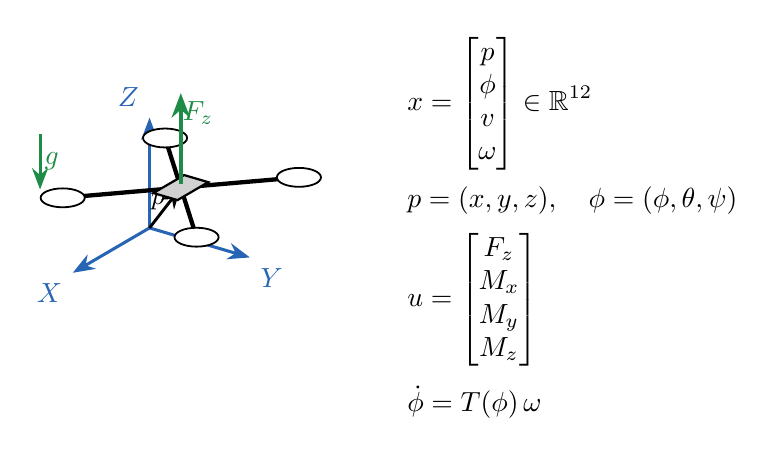
\begin{tikzpicture}[>=Stealth, font=\normalsize]
  \definecolor{Wcol}{RGB}{40,100,180}
  \definecolor{Fcol}{RGB}{30,140,70}

  % world frame
  \draw[->, Wcol, line width=1.1pt] \xyz{0}{0}{0} -- \xyz{1.5}{0}{0}
    node[anchor=north east] {$X$};
  \draw[->, Wcol, line width=1.1pt] \xyz{0}{0}{0} -- \xyz{0}{1.5}{0}
    node[anchor=north west] {$Y$};
  \draw[->, Wcol, line width=1.1pt] \xyz{0}{0}{0} -- \xyz{0}{0}{1.4}
    node[anchor=south east] {$Z$};

  % vehicle
  \def\px{1.35}
  \def\py{1.50}
  \def\pz{1.40}
  \def\L{1.00}
  \path \xyz{\px}{\py}{\pz} coordinate (P);

  \draw[->, black, line width=1.05pt] \xyz{0}{0}{0} -- (P);
  \node[anchor=south] at \xyz{0.55}{0.55}{0.45} {$p$};

  \draw[black, line width=1.55pt]
    \xyz{\px-\L}{\py-\L}{\pz} -- \xyz{\px+\L}{\py+\L}{\pz};
  \draw[black, line width=1.55pt]
    \xyz{\px-\L}{\py+\L}{\pz} -- \xyz{\px+\L}{\py-\L}{\pz};
  \filldraw[fill=black!18, draw=black, line width=0.8pt]
    \xyz{\px-0.30}{\py-0.18}{\pz} --
    \xyz{\px+0.30}{\py-0.18}{\pz} --
    \xyz{\px+0.30}{\py+0.18}{\pz} --
    \xyz{\px-0.30}{\py+0.18}{\pz} -- cycle;
  \foreach \sx/\sy in {-1/-1,1/1,-1/1,1/-1} {
    \filldraw[fill=white, draw=black, line width=0.65pt]
      \xyz{\px+\sx*\L}{\py+\sy*\L}{\pz} ellipse (0.28 and 0.12);
  }

  % Fz up, g aside — plenty of clearance
  \draw[->, Fcol, line width=1.3pt]
    \xyz{\px}{\py}{\pz+0.05} -- \xyz{\px}{\py}{\pz+1.20};
  \node[Fcol, anchor=west] at \xyz{\px+0.15}{\py}{\pz+1.00} {$F_z$};

  \draw[->, Fcol, line width=1.05pt]
    \xyz{2.40}{0.20}{2.15} -- \xyz{2.40}{0.20}{1.45};
  \node[Fcol, anchor=west] at \xyz{2.50}{0.20}{1.85} {$g$};

  % formulas only — attitude detailed in math, not on drawing
  \node[anchor=north west, align=left] at (3.15,2.55) {%
    $\displaystyle
      x=\begin{bmatrix}p\\ \phi\\ v\\ \omega\end{bmatrix}
      \in\mathbb{R}^{12}
    $\\[5pt]
    $p=(x,y,z),\quad
     \phi=(\phi,\theta,\psi)$\\[6pt]
    $\displaystyle
      u=\begin{bmatrix}F_z\\ M_x\\ M_y\\ M_z\end{bmatrix}
    $\\[6pt]
    $\displaystyle \dot{\phi}=T(\phi)\,\omega$%
  };
\end{tikzpicture}
\end{document}
